\documentclass[9pt]{beamer}

%~~~~~~~~~~~~~~~~~~~~~~~~~~~~~~~~~~~~~~~~~~~~~~~~~~~~~~~~~~~~~~~~~~~~~~~~~~~~~~
% Use roboto Font (recommended)
\usepackage[sfdefault]{roboto}
\usepackage[utf8]{inputenc}
\usepackage[T1]{fontenc}
%~~~~~~~~~~~~~~~~~~~~~~~~~~~~~~~~~~~~~~~~~~~~~~~~~~~~~~~~~~~~~~~~~~~~~~~~~~~~~~

%~~~~~~~~~~~~~~~~~~~~~~~~~~~~~~~~~~~~~~~~~~~~~~~~~~~~~~~~~~~~~~~~~~~~~~~~~~~~~~
% Define where theme files are located. ('/styles')
\usepackage{styles/fluxmacros}
\usefolder{styles}
% Use Flux theme v0.1 beta
% Available style: asphalt, blue, red, green, gray 
\usetheme[style=mpik]{flux}
%~~~~~~~~~~~~~~~~~~~~~~~~~~~~~~~~~~~~~~~~~~~~~~~~~~~~~~~~~~~~~~~~~~~~~~~~~~~~~~

%~~~~~~~~~~~~~~~~~~~~~~~~~~~~~~~~~~~~~~~~~~~~~~~~~~~~~~~~~~~~~~~~~~~~~~~~~~~~~~
% Extra packages for the demo:
\usepackage{booktabs}
\usepackage{colortbl}
\usepackage{ragged2e}
\usepackage{schemabloc}
\usepackage{mathpazo}
%~~~~~~~~~~~~~~~~~~~~~~~~~~~~~~~~~~~~~~~~~~~~~~~~~~~~~~~~~~~~~~~~~~~~~~~~~~~~~~

%~~~~~~~~~~~~~~~~~~~~~~~~~~~~~~~~~~~~~~~~~~~~~~~~~~~~~~~~~~~~~~~~~~~~~~~~~~~~~~
% Special maths fonts:
\usepackage{mathpazo}
%\usepackage{euler}
%~~~~~~~~~~~~~~~~~~~~~~~~~~~~~~~~~~~~~~~~~~~~~~~~~~~~~~~~~~~~~~~~~~~~~~~~~~~~~~
\usepackage{pdfpages}
\usepackage{xspace}
\usepackage{morefloats,subfig,afterpage,mathtools,slashed,mathrsfs,slashed}
\usepackage{graphicx}
\usepackage{listings}
\usepackage{epstopdf}
\usepackage{multirow,multicol}
%\usepackage{float}  
\usepackage{cite} 
\usepackage{amsfonts}

%\usepackage{geometry}
\usepackage{pgfplotstable}
\usepackage{array}
\usepackage{booktabs}
\usepackage{pgfplots, pgfplotstable}
%\geometry{
%	paper = a4paper , % Change to letterpaper for US letter
%	inner = \dimexpr0.5in+33pt\relax , % Inner margin
%	outer = \dimexpr0.5in+22pt\relax , % Outer margin
%	top = \dimexpr1in+12pt+24pt\relax , % Top margin
%	bottom = \dimexpr 1in+24pt\relax, % Bottom margin
%	marginpar = 51pt ,
%	marginparsep = 17pt ,
%	foot = 24pt ,
%	headsep = 24pt
%}
%\usepackage{showkeys}
%\usepackage[]{latexsym}
%\usepackage{}
%\graphicspath{./figures/}
%% Using Babel allows other languages to be used and mixed-in easily
%\usepackage[ngerman,english]{babel}


%% Citation system tweaks
% \let\@OldCite\cite
% \renewcommand{\cite}[1]{\mbox{\!\!\!\@OldCite{#1}}}

%% Maths
% TODO: rework or eliminate maybemath
\usepackage{abmath}
\DeclareRobustCommand{\mymath}[1]{\ensuremath{\maybebmsf{#1}}}
\DeclareRobustCommand{\parenths}[1]{\mymath{\left({#1}\right)}\xspace}
\DeclareRobustCommand{\braces}[1]{\mymath{\left\{{#1}\right\}}\xspace}
% \DeclareRobustCommand{\angles}[1]{\mymath{\left\langle{#1}\right\rangle}\xspace}
\DeclareRobustCommand{\sqbracs}[1]{\mymath{\left[{#1}\right]}\xspace}
\DeclareRobustCommand{\mods}[1]{\mymath{\left\lvert{#1}\right\rvert}\xspace}
\DeclareRobustCommand{\modsq}[1]{\mymath{\mods{#1}^2}\xspace}
 \DeclareRobustCommand{\dblmods}[1]{\mymath{\left\lVert{#1}\right\rVert}\xspace}
 \DeclareRobustCommand{\expOf}[1]{\mymath{\exp{\!\parenths{#1}}}\xspace}
 \DeclareRobustCommand{\eexp}[1]{e^{#1}\xspace}
 \DeclareRobustCommand{\plusquad}{\mymath{\oplus}\xspace}
 \DeclareRobustCommand{\logOf}[1]{\mymath{\log\!\parenths{#1}}\xspace}
 \DeclareRobustCommand{\lnOf}[1]{\mymath{\ln\!\parenths{#1}}\xspace}
\DeclareRobustCommand{\ofOrder}[1]{\mymath{\mathcal{O}\parenths{#1}}\xspace}
\DeclareRobustCommand{\SOgroup}[1]{\mymath{\mathup{SO}\parenths{#1}}\xspace}
\DeclareRobustCommand{\SUgroup}[1]{\mymath{\mathup{SU}\parenths{#1}}\xspace}
\DeclareRobustCommand{\Ugroup}[1]{\mymath{\mathup{U}\parenths{#1}}\xspace}
%\DeclareRobustCommand{\I}[1]{\mymath{\mathrm{i}}\xspace}
\DeclareRobustCommand{\colvector}[1]{\mymath{\begin{pmatrix}#1\end{pmatrix}}\xspace}
\DeclareRobustCommand{\Rate}{\mymath{\Gamma}\xspace}
\DeclareRobustCommand{\RateOf}[1]{\mymath{\Gamma}\parenths{#1}\xspace}
\DeclareRobustCommand{\pt}{p_{T}}
\DeclareRobustCommand{\fOf}[1]{\mymath{f_{\text{#1}}\xspace}}
\DeclareRobustCommand{\ToThe}[2]{\mymath{#1\cdot 10^{#2}}}
\DeclareRobustCommand{\sqrts}{\sqrt{s}\xspace}
\DeclareRobustCommand{\intlum}{\int \mathscr L dt}
\newcommand{\E}[1]{\mbox{$\cdot 10^{#1}$}}
\DeclareRobustCommand{\bra}[1]{\mbox{$\langle\, #1 \mid$}}
\newcommand{\bbra}[1]{\mbox{$\left\langle\, #1 \right\mid$}}
\DeclareRobustCommand{\ket}[1]{\mbox{$\mid #1\,\rangle$}}
\newcommand{\bket}[1]{\mbox{$\left\mid #1\,\right\rangle$}}
\newcommand{\pro}[2]{\mbox{$\langle\, #1 \mid #2\,\rangle$}}
\newcommand{\expec}[1]{\mbox{$\langle\, #1\,\rangle$}}
\newcommand{\expecl}[1]{\mbox{$\left\langle\,\strut\displaystyle{#1}\,\right\rangle$}}
\newcommand{\be}{\begin{eqnarray}}
\newcommand{\ee}{\end{eqnarray}}
\newcommand{\bea}{\begin{eqnarray}}
\newcommand{\eea}{\end{eqnarray}}
%%% High-energy physics stuff
%\usepackage{abhep}
%\usepackage{hepnames}
\usepackage{hepunits}
\DeclareRobustCommand{\arXivCode}[1]{arXiv:#1}
\DeclareRobustCommand{\CP}{\ensuremath{\mathcal{CP}}\xspace}
\DeclareRobustCommand{\CPviolation}{\CP-violation\xspace}
\DeclareRobustCommand{\CPv}{\CPviolation}
\DeclareRobustCommand{\LHCb}{LHCb\xspace}
\DeclareRobustCommand{\LHC}{LHC\xspace}
\DeclareRobustCommand{\LEP}{LEP\xspace}
\DeclareRobustCommand{\CERN}{CERN\xspace}
\DeclareRobustCommand{\VELO}{VELO\xspace}
%\DeclareRobustCommand{\bphysics}{\Pbottom-physics\xspace}
%\DeclareRobustCommand{\bhadron}{\Pbottom-hadron\xspace}
%\DeclareRobustCommand{\Bmeson}{\PB-meson\xspace}
%\DeclareRobustCommand{\bbaryon}{\Pbottom-baryon\xspace}
%\DeclareRobustCommand{\Bdecay}{\PB-decay\xspace}
%\DeclareRobustCommand{\bdecay}{\Pbottom-decay\xspace}
%\DeclareRobustCommand{\BToKPi}{\HepProcess{ \PB \to \PK \Ppi }\xspace}
%\DeclareRobustCommand{\BToPiPi}{\HepProcess{ \PB \to \Ppi \Ppi }\xspace}
%\DeclareRobustCommand{\BToKK}{\HepProcess{ \PB \to \PK \PK }\xspace}
%\DeclareRobustCommand{\BToRhoPi}{\HepProcess{ \PB \to \Prho \Ppi }\xspace}
%\DeclareRobustCommand{\BToRhoRho}{\HepProcess{ \PB \to \Prho \Prho }\xspace}
%\DeclareRobustCommand{\BToKll}{\HepProcess{ \PB \to \PKstar(892) \Plepton \Plepton }\xspace}
%\DeclareRobustCommand{\BToKtt}{\HepProcess{ \PB \to \PKstar(892) \tau^- \tau^+ }\xspace}
%\DeclareRobustCommand{\BToKmm}{\HepProcess{ \PB \to \PKstar(892) \Pmuon  \APmuon  }\xspace}
%\DeclareRobustCommand{\BToKee}{\HepProcess{ \PB \to \PKstar(892) \Pelectron \APelectron }\xspace}
%\DeclareRobustCommand{\X}{\thesismath{X}\xspace}
%\DeclareRobustCommand{\Xbar}{\thesismath{\overline{X}}\xspace}
%\DeclareRobustCommand{\Xzero}{\HepGenParticle{X}{}{0}\xspace}
%\DeclareRobustCommand{\Xzerobar}{\HepGenAntiParticle{X}{}{0}\xspace}
%\DeclareRobustCommand{\epluseminus}{\Ppositron\!\Pelectron\xspace}
%\DeclareRobustCommand{\protonproton}{\Pproton\APantiproton\xspace}

\definecolor{mygreen}{rgb}{0,0.6,0}
\definecolor{mygray}{rgb}{0.5,0.5,0.5}
\definecolor{mymauve}{rgb}{0.58,0,0.82}
\lstset{ %
	backgroundcolor=\color{white},   % choose the background color
	basicstyle=\footnotesize,        % size of fonts used for the code
	breaklines=true,                 % automatic line breaking only at whitespace
	captionpos=b,                    % sets the caption-position to bottom
	commentstyle=\color{mygreen},    % comment style
	escapeinside={\%*}{*)},          % if you want to add LaTeX within your code
	keywordstyle=\color{blue},       % keyword style
	stringstyle=\color{mymauve},     % string literal style
}

%\definecolor{dkgreen}{rgb}{0,0.6,0}
%\definecolor{gray}{rgb}{0.5,0.5,0.5}
%\definecolor{mauve}{rgb}{0.58,0,0.82}
%\lstset{frame=tb,
%	language=c++,
%	aboveskip=3mm,
%	belowskip=3mm,
%	showstringspaces=false,
%	columns=flexible,
%	basicstyle={\small\ttfamily},
%	numbers=none,
%	numberstyle=\tiny\color{gray},
%	keywordstyle=\color{blue},
%	commentstyle=\color{dkgreen},
%	stringstyle=\color{mauve},
%	breaklines=true,
%	breakatwhitespace=true,
%	tabsize=3
%}
%~~~~~~~~~~~~~~~~~~~~~~~~~~~~~~~~~~~~~~~~~~~~~~~~~~~~~~~~~~~~~~~~~~~~~~~~~~~~~~
% Information
\title{My beamer template}
\subtitle{for MPIK, modified from FLUX style}
\author{Lina Alasfar}
\institute{Max-Planck-Institute for Nuclear Physics, Heildelberg\\ LHCb Collabouration }
\date{\today}
\titlegraphic{assets/mpik.png}
%~~~~~~~~~~~~~~~~~~~~~~~~~~~~~~~~~~~~~~~~~~~~~~~~~~~~~~~~~~~~~~~~~~~~~~~~~~~~~~

\begin{document}

% Generate title page
\titlepage

\begin{frame}
 \frametitle{Table of contents}
 \tableofcontents
\end{frame}

\section{Presentation}

\subsection{introduction}

\begin{frame}{Flux}{introduction}
	\justifying
 Flux is a modern style beamer presentation. It is provided as a work in progress version and may suffer from inconsistencies. Sources and complementary information are available at\\[0.3cm]
 	\centering\textbf{github.com/pvanberg/flux-beamer}
\end{frame}

\def\beamer@mytheme@style{green}
\begin{frame}[fragile]{Flux}{colors}
	\centering
	Flux provides five different color palettes.\\
	\verb+\usetheme[style=asphalt]{flux}+\\[0.8cm]
	\newcommand{\colorRow}[1]{
	\begin{tabular}{p{4cm}cccc}
	#1 & \cellcolor{primary}\hspace*{1cm} &\cellcolor{primaryLight}\hspace*{1cm}&\cellcolor{secondary}\hspace*{1cm}&\cellcolor{tertiary}\hspace*{1cm}\\
 	\end{tabular}
 	}
 	\colorRow{Asphalt}\\[0.3cm]
	\definecolor{primaryLight}{HTML}{3A99D9}
	\definecolor{primary}{HTML}{2E81B7}
	\definecolor{secondary}{HTML}{2E81B7}
	\definecolor{tertiary}{HTML}{E76D55}
 	\colorRow{Blue}\\[0.3cm]
    \definecolor{primaryLight}{HTML}{77933C}
    \definecolor{primary}{HTML}{4F622A}
    \definecolor{secondary}{HTML}{884F4D}
    \definecolor{tertiary}{HTML}{2B3234}
 	\colorRow{Green}\\[0.3cm]
 	\definecolor{primaryLight}{HTML}{C0392B}
    \definecolor{primary}{HTML}{96281B}
    \definecolor{secondary}{HTML}{347986}
    \definecolor{tertiary}{HTML}{56423E}
 	\colorRow{Red}\\[0.3cm]
 	\definecolor{primaryLight}{HTML}{616161}
	\definecolor{primary}{HTML}{424242}
	\definecolor{secondary}{HTML}{518071}
	\definecolor{tertiary}{HTML}{8B7687}
 	\colorRow{Gray}\\[0.3cm]
\end{frame}

\subsection{fonts}

\begin{frame}[fragile]{Flux}{fonts}
 Flux recommends the use of Roboto or Overpass font and a font size of 9pt.\\[0.2cm]
 \begin{center}
 	\verb+\documentclass[9pt]{beamer}+\\
	\verb+\usepackage[sfdefault]{roboto}+
 \end{center}
 
  Flux also implements default typographies.

	\begin{itemize}
		\item Regular
		\item \alert{Alert}
		\item \example{Example}
		\item \textit{Italic}
		\item \textbf{Bold}
	\end{itemize}
	
\end{frame}

\subsection{footnotes}

\begin{frame}{Flux}{footnotes}
		Flux also includes custom footnote integration. For instance, this \textbf{element}\footnote{Footnotes are notes placed at the bottom of a page. They cite references or comment on a designated part of the text above it. For example, say you want to add an interesting comment to a sentence you have written, but the comment is not directly related to the argument of your paragraph. } and this \textbf{element}\footnote{Footnotes are not just for interesting comments, however. Sometimes they simply refer to relevant sources -- they let your reader know where certain material came from, or where they can look for other sources on the subject.} provide a footnote.
\end{frame}

\section{Collections}
\subsection{lists}

\begin{frame}{Flux}{lists}
   \begin{columns}[T,onlytextwidth]
    \column{0.33\textwidth}
      \textbf{Items}
      \begin{itemize}
        \item Cats \item Dogs \item Birds
      \end{itemize}

    \column{0.33\textwidth}
      \textbf{Enumerations}
      \begin{enumerate}
        \item First \item Second \item Last
      \end{enumerate}

    \column{0.33\textwidth}
      \textbf{Descriptions}
      \begin{description}
        \item[Apples] Yes \item[Oranges] No \item[Grappes] No
      \end{description}
\end{columns}
\let\thefootnote\relax\footnote{Note the following demo slides are directly taken from metropolis theme. Copyright 2014 Matthias Vogelgesang.\\
Give a look at https://github.com/matze/mtheme/tree/master/demo}
\end{frame}

\subsection{tables}

\begin{frame}{Flux}{tables}
  \begin{table}
    \caption{Largest cities in the world (source: Wikipedia)}
    \begin{tabular}{@{} lr @{}}
      \toprule
      City & Population\\
      \midrule
      Mexico City & 20,116,842\\
      Shanghai & 19,210,000\\
      Peking & 15,796,450\\
      Istanbul & 14,160,467\\
      \bottomrule
    \end{tabular}
    \hspace*{1cm}
        \setlength\extrarowheight{3pt}
    \begin{tabular}{|lr|}
      \hline
      \rowcolor{primaryLight}\color{background}City & \color{background}Population\\
      \hline
      Mexico City & 20,116,842\\
      Shanghai & 19,210,000\\
      Peking & 15,796,450\\
      Istanbul & 14,160,467\\
      \hline
    \end{tabular}
\end{table}
\end{frame}

\subsection{blocs}

\begin{frame}[fragile]{Flux}{blocks}
  		Flux theme comes with three pre-defined block style collections.\\
  		Native style (default) available as \verb+\setblockstyle{native}+\\[0.5cm]
  
   \setblockstyle{native} % Default behavior, optional line.
   \centering
	\begin{minipage}[b]{0.5\textwidth}

	  \begin{block}{Default}
        Block content.
      \end{block}

      \begin{alertblock}{Alert}
        Block content.
      \end{alertblock}

      \begin{exampleblock}{Example}
        Block content.
      \end{exampleblock}      
      
	\end{minipage}
	
\end{frame}

\begin{frame}[fragile]{Flux}{blocks}
  		Flux theme comes with three pre-defined block style collections.\\
  		NoBackground style available as \verb+\setblockstyle{nobackground}+\\[0.5cm]
  
   \setblockstyle{nobackground}
   \centering
	\begin{minipage}[b]{0.5\textwidth}

	  \begin{block}{Default}
        Block content.
      \end{block}

      \begin{alertblock}{Alert}
        Block content.
      \end{alertblock}

      \begin{exampleblock}{Example}
        Block content.
      \end{exampleblock}       
      
	\end{minipage}
	
\end{frame}

\begin{frame}[fragile]{Flux}{blocks}
  		Flux theme comes with three pre-defined block style collections.\\
  		Metropolis style available as \verb+\setblockstyle{metropolis}+\\[0.5cm]
  
   \setblockstyle{metropolis}
   \centering
	\begin{minipage}[b]{0.5\textwidth}

	  \begin{block}{Default}
        Block content.
      \end{block}

      \begin{alertblock}{Alert}
        Block content.
      \end{alertblock}

      \begin{exampleblock}{Example}
        Block content.
      \end{exampleblock}      
      
	\end{minipage}
	
\end{frame}

\begin{frame}{Flux}{diagrams}
\centering
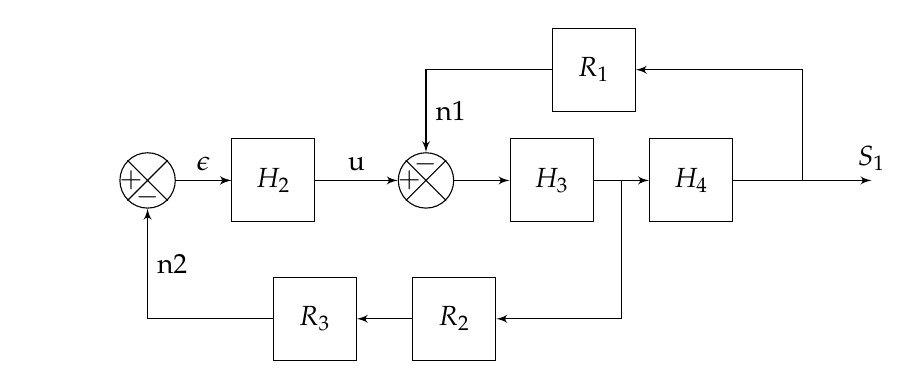
\begin{tikzpicture}
    \sbEntree{E}
    \sbComp{a}{E}
    \sbBlocL{c}{$H_2$}{a}
            \sbRelier[$\epsilon$]{a}{c}
    \sbComph{d}{c}
            \sbRelier[u]{c}{d}
    \sbBlocL{e}{$H_3$}{d}
    \sbBlocL{f}{$H_4$}{e}
    \sbSortie[5]{S1}{f}
            \sbRelier{f}{S1}
            \sbNomLien[0.8]{S1}{$S_1$}
    \sbDecaleNoeudy[-4]{f}{u}
    \sbDecaleNoeudy{e}{v}
    \sbBlocr{r1}{$R_1$}{u}
    \sbBlocr{r2}{$R_2$}{v}
    \sbBlocrL{r3}{$R_3$}{r2}
    \sbRelieryx{f-S1}{r1}
    \sbRelierxy[n1]{r1}{d}
    \sbRelieryx{e-f}{r2}
    \sbRelierxy[n2]{r3}{a}
\end{tikzpicture}\\[0.4cm]
Bloc diagram example from \textbf{texample.net}
\end{frame}

\begin{frame}{Flux}{plots}
	\begin{minipage}{0.56\textwidth}
		\begin{figure}
			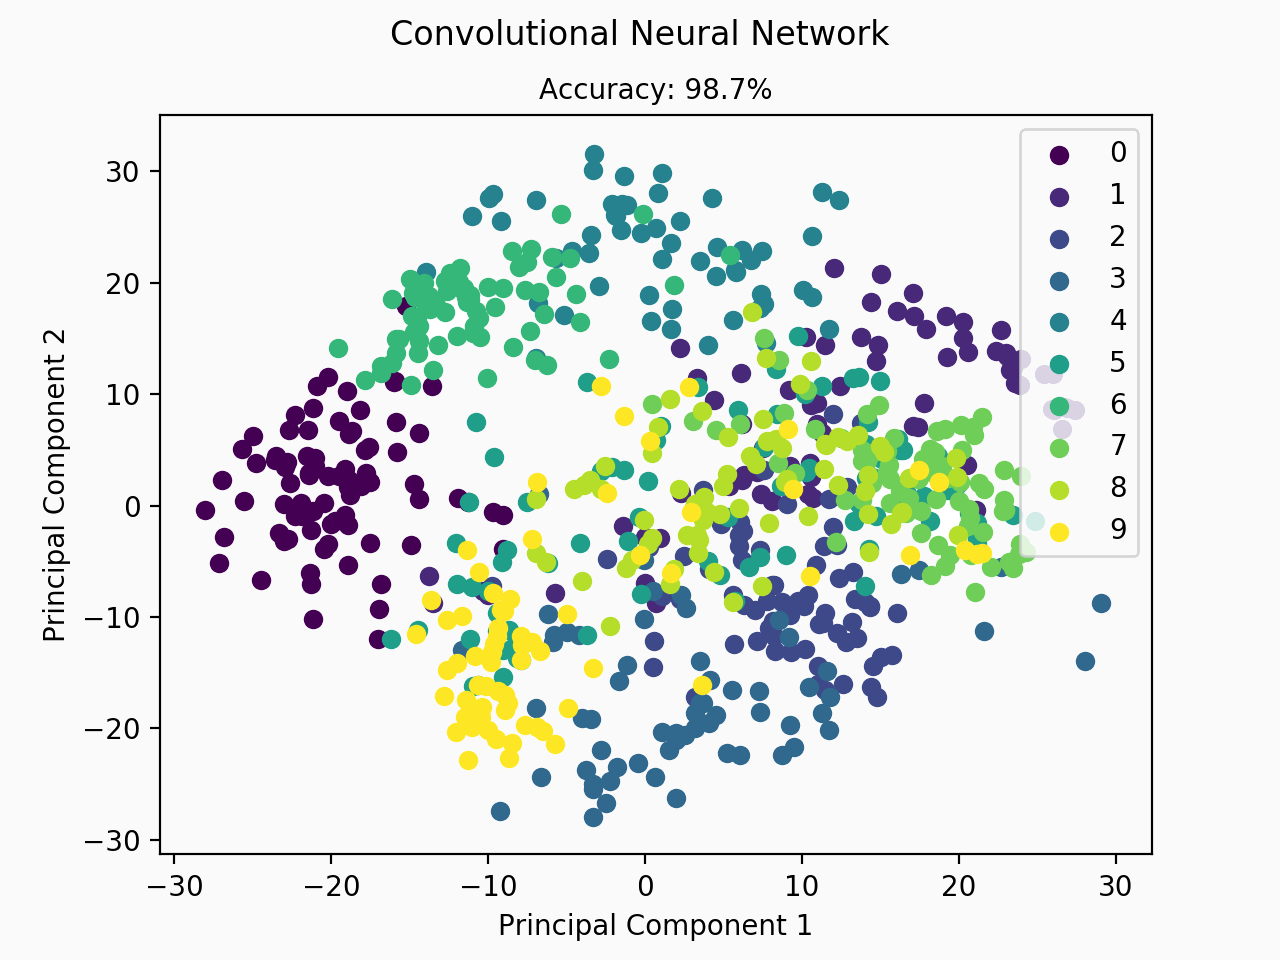
\includegraphics[width=\textwidth]{assets/plot.png}
		\end{figure}
	\end{minipage}
	\hfill
	\begin{minipage}{0.38\textwidth}
		\begin{block}{Binary Softmax classifier}
			\centering
			$\sigma(\sum_i w_ix_i + b)$
		\end{block}
		\begin{exampleblock}{Loss function}
			\centering\vspace*{0.1cm}
			$L_i = -log(\frac{e^{f_{y_i}}}{\sum_j e^{f_j}})$\\[0.1cm]
			cross entropy
		\end{exampleblock}
	\end{minipage}
\end{frame}

% The [plain] causes the headlines, footlines, and sidebars 
% to be suppressed. Useful for showing large pictures
\begin{frame}[plain]
	\begin{center}
	  This is a plain frame.\\
	  Use it to display full page images.
	  \end{center}
\end{frame}

\begin{frame}[allowframebreaks]{References}

  \nocite{*}
  \bibliography{demo}
  \bibliographystyle{abbrv}

\end{frame}

\section{Next section}
\subsection{subsection 1}
\subsection{subsection 2}
\subsection{subsection 3}
\section{One more section}
\subsection{subsection 1}
\subsection{subsection 2}
\subsection{subsection 3}

\begin{frame}
 \centering
 \frametitle{Flux}
 \framesubtitle{license}
 Flux is licensed under GNU General Public License v3.\\[0.3cm]
 	\centering\textbf{http://www.gnu.org/licenses}\\[0.3cm]
Inspired by \textbf{Metropolis} theme from Matthias Vogelgesang.\\
https://github.com/matze/mtheme 
 
\end{frame}

\end{document}